\documentclass[10pt]{beamer}

\usepackage{appendixnumberbeamer}

\usepackage{booktabs}
\usepackage[scale=2]{ccicons}

\usepackage{pgfplots}
\usepgfplotslibrary{dateplot}

\usepackage{xspace}
\usepackage{../theme_style}
\setbeameroption{show notes on second screen}

\title[Fault tolerance and consensus]{Exam question 3 - Fault tolerance and consensus}
\subtitle{Distributed and Pervasive Systems}
\date{June 03, 2022}
\author[M.H. Kristensen]{Morten Haahr Kristensen}
\def\studentid{201807664}
\institute{Department of Electrical and Computer Engineering - Aarhus University}
% Logo only on title page
\titlegraphic{
    
\includegraphics[width=12cm]{figs/aulogo_big.png}
}
\begin{document}

\maketitle

\begin{frame}{Outline}
  \setbeamertemplate{section in toc}[sections numbered]
  \tableofcontents[hideallsubsections]
\end{frame}

\section{Motivation}
\begin{frame}{Motivation}
  \metroset{block=fill}
  \begin{alertblock}{Distributed System definition\cite{vansteenDistributedSystems2018}}
    A distributed system is a collection of autonomous computing elements that \textbf{appears} to its users as \textbf{a single coherent system}.
    \note[item]{
      There are many advantages to distributed systems. E.g. horizontal scaling, compute pricing, parallel computation etc.\\
      The disadvantages however all relate in one way or another to the added complexity.
    }
  \end{alertblock}
  \begin{itemize}
    \item Benefit of distributed systems: Fault tolerance through redundancy.
    \note[item]{The overall system can become more robust if we have redundancy. If a single node fails then the others can take over. The redundancy can both be considered a blessing and a curse. A blessing because the system can become much more stable and a curse because it can now fail in new and challenging ways.}
    \item Distributed systems can have partial failures.
    \note[item]{A partial failure is a failure that leaves the system in an operational state. One of the things I will be going in-depth with today is how to recover from these failures and provide fault tolerance.}
  \end{itemize}
\end{frame}

\section{Fault tolerance}
\begin{frame}
  \frametitle{Overview}
  A system's ability to recover from partial failures.

  Metrics:
  \begin{itemize}
    \item \alert{Availability}
    \item \alert{Reliability}
    \item \alert{Safety}
    \item Maintainability
  \end{itemize}
  \note{Availability: The probability that the system is operating correctly at any given time.\\
  Reliability: The average time span that the system runs continuously without failure.\\
  Availability vs Reliability: A system that crashes for 1s every hour has great availability but low reliability. It is available 99.9 \% of the time but it is unreliable as it crashes every hour.\\
  Safety: If the system fails, does a catastrophe happen? This might at first glance not seem very related to DS but if we have a recovery system where the system gracefully shuts down when a majority of the nodes have failed it might prevent a catastrophe.\\
  Maintainability: A DS may or may not be easier to maintain than a centralized system. I would guess in most cases it is harder but it is very application-specific. Lunar argues it is easier if you have a microservices architecture.}
  Keyword: \textbf{Redundancy.}
\end{frame}

\begin{frame}
  \frametitle{Failure types}
  Categorized failure types in distributed systems: \cite{pedersenFaultToleranceConsensus2022}
  \begin{itemize}
    \item Crash failure
    \item Omission failure
    \begin{itemize}
      \item Receive omission
      \item Send omission
    \end{itemize}
    \item Timing failure
    \item Response failure
    \begin{itemize}
      \item Value failure
      \item State-transition failure
    \end{itemize}
    \item Byzantine failure
  \end{itemize}
  \note{
    Crash failure: Basically BSOD in Windows systems. Everything is fine but then the system crashes and needs a reboot.\\
    Omission failure: Fails to respond to incoming requests. Two types:\\
    Receive omission: Fails to receive messages.\\
    Send omission: Fails to send messages.\\
    Timing failure: Response is either sent too early or too late.\\
    Response failure: Incorrect response. Two types:\\
    Value failure: The value is wrong.\\
    State-transition failure: Somehow enters a wrong state.\\
    Byzantine failure: One or more nodes have failed but there is no information to indicate this and no information indicating that the system is incorrect. This is the worst type of error.
  }
\end{frame}

\begin{frame}
  \frametitle{Consensus}

  Problem with redundancy: Nodes must achieve \textbf{consensus}.
  \note{Consensus means that all the nodes agree on some value. The value could also be a state that the system is in. For a distributed system to appear as a single coherent system it doesn't make sense if the nodes disagree on their state.}
  
  Consensus is achieved through a consensus algorithm.
\end{frame}

\section{RAFT}

\begin{frame}
  \frametitle{RAFT components}
  Three main points:
  \begin{itemize}
    \item Leader election
    \item Log replication
    \item Safety
  \end{itemize}
  \note{
    Leader election: One node must take the role of leader for the system to progress. The leader is selected when the previous node crashes.\\
    Log replication: This is our normal operation state. Here the leader takes commands from the client and appends them to its log. It will try to get the commands committed by replicating them to at least half of the nodes.\\
    Safety: During leader election, nodes only vote for other nodes whose logs are considered more up to date. Logs are only committed when a majority of the system is in consensus regarding the log. Responses are only sent once a request is committed.
  }
\end{frame}

\begin{frame}
  \frametitle{Leader election - initial}
  \begin{figure}
    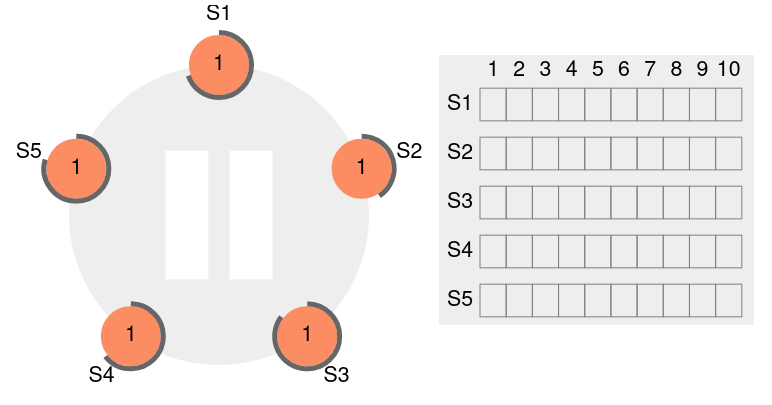
\includegraphics[width=0.8\textwidth]{figs/raft_initial.png}
    \caption{Initial leader election about to start.\cite{ongaroRaftScope2014}}
  \end{figure}
  \vspace*{-1.5em}
  \begin{itemize}
    \small
    \item 5 servers
    \item Timers
    \item Same term
  \end{itemize}
  \note{This could be an example of how leader election might initially look like. In this example we have 5 servers in a distributed system. Since the system just booted they are all currently ''followers'' and they are waiting for a heartbeat from a leader. The leader obviously doesn't exist so once the shortest timer on S2 runs out one of them will increment its term count and hold an election. The duration of the timers are randomized between two time intervals to avoid the probability of two simultaneous elections occuring.\\
  Another solution could be to rank the servers but the authors found the timer solution to be less confusing which is one of the main goals for RAFT - to be simple to understand.}
\end{frame}


\begin{frame}
  \frametitle{Leader election - ongoing}
  \begin{figure}
    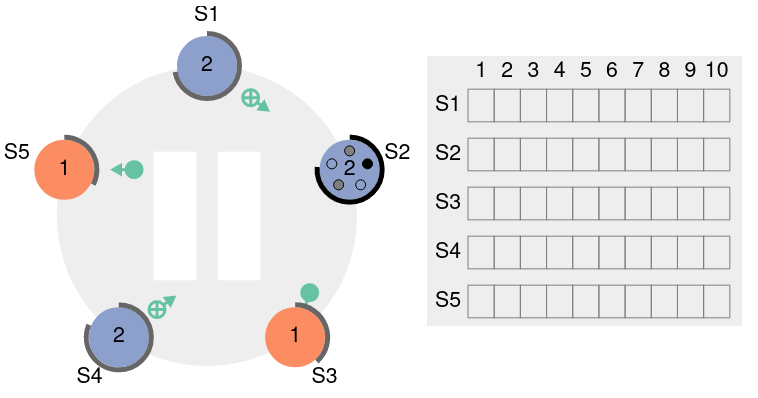
\includegraphics[width=0.8\textwidth]{figs/raft_initial_election.png}
    \caption{Server two has started an election.\cite{ongaroRaftScope2014}}
  \end{figure}
  \vspace*{-1.5em}
  \begin{itemize}
    \small
    \item Dots on server 2
    \item Ingoing/outgoing requests
    \item Voters increase their terms (if they vote for the candidate)
  \end{itemize}
  \note{So here we can see that server 2 has started an election. It has incremented the term count and promoted itself to candidate. It then sends RequestVote messages (remote procedure calls) to the followers where hopefully it gets elected. This is what we see on the image as green circles. We see that S1 and S4 are sending their acknowledgments to S2 as a leader and S5 and S3 haven't received the requests yet but they will also agree. The reason for a server to not acknowledge the candidate would be if the candidate's term was not higher than their own. I will elaborate further on these rules when talking about safety.}
\end{frame}

\begin{frame}
  \frametitle{Log replication}
  Idea:
  \begin{itemize}
    \item Deterministic state machine
    \note[item]{
    The overall system can be seen as a deterministic state machine.\\
    Difference between deterministic and non-deterministic state machines: With deterministic the new state is completely determined by the input (not a combination of the input and e.g. something external like temperature) and the state never changes without input.
  }
    \item Client requests considered as log entries
    \item Response received once entry is committed among the majority
  \end{itemize}
  
  Procedure:
  \begin{enumerate}
    \item Leader receives a command from a client
    \item Leader appends to its log and sends AppendEntries to followers. Continues until the majority agrees on the log
    \item Leader marks the entry as committed among itself and followers
    \note[item]{
      The leader marks the entry as committed by sending more requests to the followers.
    }
    \item Command is executed by the leader and followers
    \item Leader's response sent to the client
    \note[item]{
      Since the system is a deterministic state machine it doesn't matter who sends the response but it would make sense to have the leader return it since it also received the request.
    }
  \end{enumerate}
\end{frame}

\begin{frame}[fragile]
  \frametitle{Log consistency}
AppendEntries include \pythoninline{<index, term>} of entry preceding new ones.
\begin{figure}
  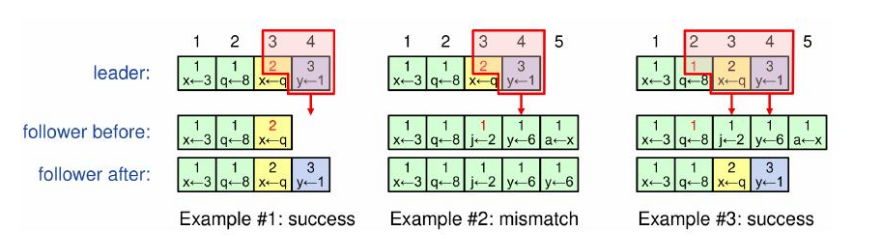
\includegraphics[width=\textwidth]{figs/log_consistency_example.png}
  \caption{Log consistency. In example \#2 the AppendEntries RPC is rejected.}
\end{figure}
\note{
  In this example, we can see that the leader is trying to append an entry to two followers. With the first follower, everything goes smoothly. The two logs are matching up until the new entry, so the follower simply acknowledges the entry request.\\
  In the second example the follower's log mismatches for some reason. Maybe it was the previous leader but had an error that disconnected it. From the AppendEntries, it can detect this mismatch since it doesn't have a matching entry from term 2. It then rejects the request.\\
  In example three the leader retries but with a longer entry list. This time it actually matches the follower's so it can be acknowledged. The follower changes its entire log to match the leader.
}
\end{frame}

\begin{frame}
  \frametitle{Safety}
  Election rules:
  \begin{itemize}
    \item Followers only vote for candidates with higher terms
    \item Followers only vote for candidates with up-to-date logs
    \begin{itemize}
      \item Ensures all committed logs will always persist
    \end{itemize}
  \end{itemize}
  
  Logs:
  \begin{itemize}
    \item Entries are only committed if a majority have the entry in their logs
  \end{itemize}

\end{frame}

\section{References}
\begin{frame}[allowframebreaks]{References}
  \bibliographystyle{ieeetr}
  \bibliography{references}
\end{frame}
\end{document}
